\documentclass[a4paper,norsk,12pt]{article}

\usepackage[norsk]{babel}
\usepackage{enumitem}
\usepackage{color}
\usepackage{amsmath}
\usepackage{amssymb}
\usepackage{wrapfig}
\usepackage{graphicx}
\usepackage[utf8]{inputenc}
\usepackage{wasysym}
\usepackage{icomma}
\usepackage{multicol}

\newcommand{\unit}[1]{~\mathrm{#1}}
\newcommand{\ans}[1]{\underline{\underline{#1}}}

\usepackage[svgnames]{xcolor}
\usepackage[most]{tcolorbox}
\usetikzlibrary{shadows}
\newcounter{exa}
\tcbset{
myexample/.style={
  enhanced,
  colback=blue!10!white,
  colframe=black,
  fonttitle=\scshape,
  titlerule=0pt,
  title={\refstepcounter{exa}Eksempel~\theexa},
  title style={fill=blue!40!white},
  coltitle=black,
  drop shadow,
  highlight math style={reset,colback=LightBlue!50!white,colframe=Navy}
  }
}

\tcbset{
mytheorem/.style={
  enhanced,
  colback=DarkGreen!10!white,
  colframe=black,
  fonttitle=\scshape,
  titlerule=0pt,
  title={Teorem},
  title style={fill=DarkGreen!40!white},
  coltitle=black,
  drop shadow,
  highlight math style={reset,colback=DarkGreen!50!white,colframe=DarkGreen}
  }
}


\tcbset{
myproof/.style={
  enhanced,
  colback=DarkGreen!10!white,
  colframe=black,
  fonttitle=\scshape,
  titlerule=0pt,
  title={Bevis},
  title style={fill=DarkGreen!40!white},
  coltitle=black,
  drop shadow,
  highlight math style={reset,colback=DarkGreen!50!white,colframe=DarkGreen}
  }
}

\tcbset{
mydef/.style={
  enhanced,
  colback=red!10!white,
  colframe=black,
  fonttitle=\scshape,
  titlerule=0pt,
  title={Definisjon},
  title style={fill=red!40!white},
  coltitle=black,
  drop shadow,
  highlight math style={reset,colback=red!50!white,colframe=red}
  }
}

\tcbset{
mysummary/.style={
  enhanced,
  colback=yellow!10!white,
  colframe=black,
  fonttitle=\scshape,
  titlerule=0pt,
  title={Oppsummering},
  title style={fill=yellow!40!white},
  coltitle=black,
  drop shadow,
  highlight math style={reset,colback=yellow!50!white,colframe=yellow}
  }
}



\newtcolorbox{texample}{myexample}
\newtcolorbox{ttheorem}{mytheorem}
\newtcolorbox{tproof}{myproof}
\newtcolorbox{tdef}{mydef}
\newtcolorbox{tsummary}{mysummary}

\begin{document}
\section{Komplekse tall}

\subsection{Behovet for komplekse tall}
Opp gjennom historien har tallbegrepet stadig blitt utvidet\footnote{Men dette er ikke et forsøk på å gjengi historien om hvordan utviklingen foregikk. Presentasjonen her forsøker å vise hvordan tallbegrepet naturlig kan og må utvikles, men historisk skjedde en del av stegene i andre rekkefølger.} for å møte behovet mennesker har hatt for å bruke matematikk til å organisere verden. Det enkleste tallkonseptet er de \emph{naturlige tallene}. Dette er tallene vi bruker til å telle objekter med, altså $\mathbb{N} = \{1, 2, 3, \ldots\}$. Med disse tallene kan vi regne ut ting som 
\begin{align*}
	&2 + 3 = 5 \\
	&8 - 2 = 6 \\
	&5\cdot 7 = 35
\end{align*}
men vi treffer raskt på begrensninger. Dersom vi ønsker å regne ut 
\begin{displaymath}
	2-3 = ?
\end{displaymath}
finnes det ikke noe svar innen de naturlige tallene. Dette viser at de naturlige tallene ikke utgjøre et komplett system, men krever en utvidelse. Vi innfører derfor \emph{heltallene}, $\mathbb{Z} = \{\ldots, -3, -2, -1, 0, 1, 2, 3, \ldots\}$. Med denne utvidelsen kan vi regne ut at
\begin{displaymath}
	2-3 = -1
\end{displaymath}
og vi kan også regne ut enhver annen addisjon, subtraksjon og multiplikasjon mellom to heltall. Men heltallene utgjør fremdeles ikke noe komplett system, noe vi ser idet vi forsøker å dividere. Hvis vi ønsker å regne ut forholdet mellom to heltall ser vi at noen ganger blir svaret et nytt heltall,
\begin{displaymath}
	\frac{8}{2} = 4,
\end{displaymath}
men vi kan lett finne eksempler der svaret ikke er et heltall
\begin{displaymath}
	\frac{1}{2} = ?
\end{displaymath}
For å bøte på dette utvider vi systemet til de \emph{rasjonale\footnote{Ordet \emph{rasjonal} er avledet av \emph{ratio}, altså forhold, og selv om ordet har felles opphav med ordet rasjonell er det ikke noen videre sammenheng mellom ordene.} tallene}, $\mathbb{Q}$. Dette er alle tall som kan skrives på formen $\frac{a}{b}$ der $a$ og $b$ er heltall ($b\neq0$) uansett om resultatet av divisjonen blir et heltall eller ikke. Når vi har definert rasjonale tall kan vi utføre enhver addisjon, subtraksjon, multiplikasjon og divisjon mellom to rasjonale tall og forbli innenfor de rasjonale tallene. Men likevel er heller ikke de rasjonale tallene er komplett i betydningen at hvis vi gjør matematiske operasjoner med to rasjonale tall er vi garantert at svaret blir rasjonalt. Dette ser vi for eksempel dersom vi bruker Pytagoras' setning til å regne ut lengden av hypotenusen i en rettvinklet trekant der begge katetene har lengde 1. En annen måte å si dette på er at vi ønsker å finne et tall $x$ som løser ligningen
\begin{displaymath}
	x^2 = 1^2 + 1^2 = 2
\end{displaymath}
Det kan bevises at svaret av denne ligningen, som vi skriver som $\sqrt{2}$, ikke selv er et rasjonalt tall. 
\begin{comment}
\begin{tproof}
For å bevise at løsningen av ligningen $x^2 = 2$ ikke er et rasjonalt tall starter vi å anta at det er det---altså at svaret kan skrives som $x=\frac{a}{b}$. Dersom løsningen kan skrives på denne formen følger det at
\begin{align*}
	2 = \left(\frac{a}{b}\right)^2 = \frac{a^2}{b^2} \\
	2b^2 = a^2
\end{align*}
Siden $a^2 = 2b^2$ må $a^2$ nødvendigvis være et partall, men da er også $a$ selv et partall. Siden $a$ er et partall er også 
\begin{displaymath}
	\frac{a^2}{2} = b^2
\end{displaymath}
et partall. Dette viser at også $b$ er et partall. Alle partall kan faktoriseres til formen $c=2^n\cdot d$ der $n$ er et heltall $\geq 1$ og $d$ er et oddetall (ikke nødvendigvis primtall). Hvis vi forkorter bort alle felles faktorer 2 i brøken $\frac{a^2}{b^2}$ kan vi altså skrive 
\begin{displaymath}
	2 = \frac{a^2}{b^2} = \frac{u^2}{v^2}
\end{displaymath}
der enten $u$, $v$ eller begge er oddetall. Siden ligningen viser at $u^2 = 2v^2$ kan $u$ ikke være et oddetall. Men da må $u$ inneholde minst en faktor 2, slik at $u^2/2$ er et partall. Men 
\begin{displaymath}
	\frac{u^2}{2} = v^2
\end{displaymath} 
så da er også $v$ et partall. Siden vi har kommet frem til en selvmotsigelse må utgangspunktet ha vært feil, og vi kan konkludere med at ligningen $x^2=2$ ikke har en løsning som kan skrives på formen $x=\frac{a}{b}$. 
\end{tproof}
\end{comment}
Oppdagelsen at det finnes tall som ikke er rasjonale krever en ny utvidelse av tallbegrepet, og vi innfører de \emph{reelle tallene} $\mathbb{R}$. Med de reelle tallene er hele tallinjen fylt opp --- uansett hvor mye eller lite vi ønsker å endre størrelsen på et tall finnes det et nytt tall som passer. Men likevel viser det seg at heller ikke de relle tallene utgjør et komplett system. Det ser vi dersom vi forsøker å løse ligningen
\begin{displaymath}
	x^2+1 = 0
\end{displaymath}
For å løse denne ligningen trenger vi et tall som har den egenskapen at det multiplisert med seg selv blir $-1$. Ethvert reellt tall (bortsett fra 0), også de negative, blir et positivt tall når man multipliserer det med seg selv. Vi trenger altså en ny utvidelse av tallsystemet. Den nye utvidelsen introduserer tallet $i$ som er definert til å ha egenskapen at 
\begin{displaymath}
	i^2 = -1
\end{displaymath}
Tallet $i$ kan både adderes, subtraheres, multipliseres og divideres med alle reelle tall. Vi kan altså skrive tall som $2+i$, $3i$ og $\pi-2i$. Dette utvidete settet av tall kaller vi for \emph{komplekse tall}, $\mathbb{C}$. Det kan vises at de komplekse tallene er et komplett sett i den betydningen at vi skriver ned en ligning med komplekse tall som koeffisienter, vil vi aldri møte på behovet for en ny utvidelse av systemet, men vi vil finne svaret som et komplekst tall.\footnote{Merk at de reelle tallene er en undermengde av de komplekse, så det er godt mulig at svaret er et reellt tall uten at det er noen konflikt med denne påstanden.}

\subsection{Representasjoner av komplekse tall}
Siden tallet $i$ ikke ligger på tallinjen trenger vi en ekstra dimensjon for å lage en grafisk representasjon av komplekse tall. Vi utvider altså tallinjen til det \emph{komplekse plan} der vi lar den horisontale aksen representere den vanlige tallinjen---nå kalt den \emph{reelle aksen}---mens tall som er multipler av $i$ ligger på den vertikale aksen---nå kalt den \emph{imaginære aksen}. Tall som verken er reelle eller rent imaginære, f.eks. $2+i$ og $\pi - 2i$ vil ikke ligge på noen av aksene. Se figur \ref{kompleks:fig:plan} for eksempler av hvordan tall tegnes inn i det kompleke tallet.
\begin{figure}[htp]
	\begin{center}
	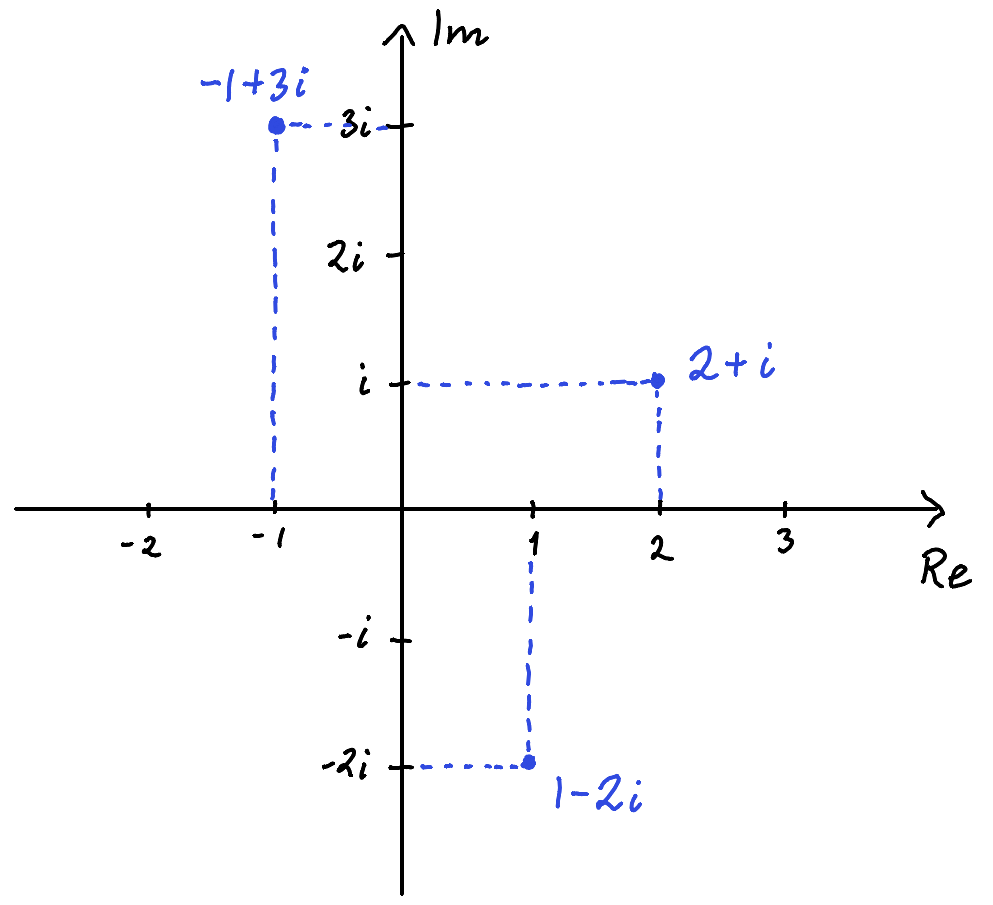
\includegraphics[width=.5\textwidth]{./standardform}
	\end{center}
	\caption{Noen tall plottet inn i det komplekse plan.}
	\label{kompleks:fig:plan}
\end{figure}

\noindent
Vi kan altså se for oss et komplekst tall som et punkt i et to-dimensjonalt plan, og vi trenger derfor to komponenter---tilsvarende $x$ og $y$ i et vanlig koordinatsystem---for å fortelle hvor tallet er. Dette gir oss det som kalles \emph{standardform}, eller noen ganger \emph{kartesisk form} av komplekse tall.

\begin{tdef}
Et komplekst tall, $z$, skrives på standardform som
\begin{displaymath}
	z = a + ib, \quad a,b\in\mathbf{R}
\end{displaymath}
\end{tdef}
\noindent
Merk at $ib = i\cdot b$, altså det ``nye'' tallet $i$ multiplisert med et reellt tall $b$. Siden faktorenes rekkefølge ikke spiller noen rolle når vi multipliserer kan vi altså like gjerne velge å skrive $z=a+bi$ (eller $z= bi + a$ for den saks skyld siden rekkefølgen heller ikke er viktig ved addisjon). Å kreve at $a$ og $b$ er reelle tall ikke er en begrensning. Anta at vi erstatter f.eks. $b$ med det komplekse tallet $c+id$, da finner vi
\begin{displaymath}
	z = a + i\cdot(c+id) = a+ ic + i^2d = a + ic +(-1)d = (a-d)+ic,
\end{displaymath}
der vi har brukt den definerende egenskapen $i^2=-1$. Vi ser altså at ``koordinatene'' alltid kan velges reelle uten å miste generalitet. 
\begin{tdef}
	Gitt det komplekse tallet $z = a+ib$. Vi kaller da $a = \mathbf{Re}(z)$ for \emph{realdelen} til $z$, og $b=\mathbf{Im}(z)$ for \emph{imaginærdelen} til $z$.
\end{tdef}
\noindent
Merk at denne definisjonen gjør at også imaginærdelen er et reelt tall; nemlig det reelle tallet som $i$ skal multipliseres med.

Siden de komplekse tallene representeres av punkter i et plan kan vi også velge å beskrive de med polarkoordinater---altså å fortelle hvor et punkt er ved å spesifisere hvor langt det er fra origo, og hvor stor vinkel forbindelseslinjen mellom origo og punktet danner med den positive realaksen ($x$-aksen). Se figur \ref{kompleks:fig:polar} for en illustrasjon av dette. 

\begin{figure}[htp]
	\begin{center}
	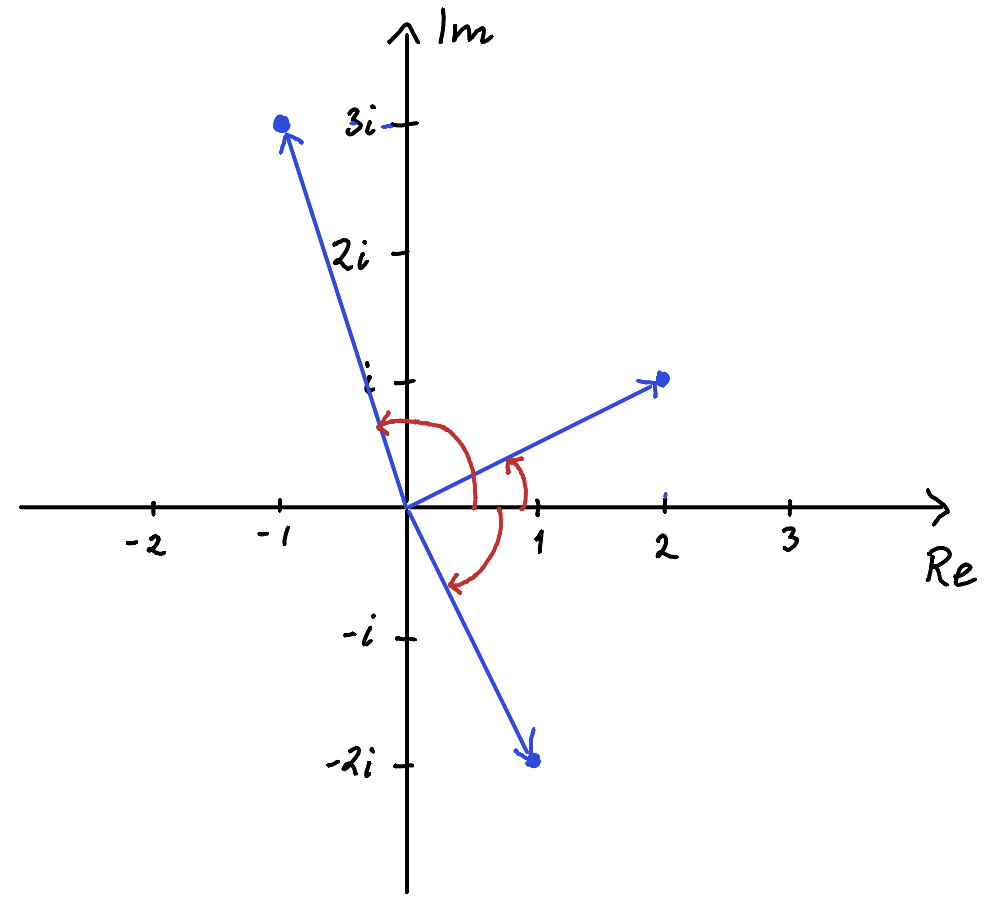
\includegraphics[width=.5\textwidth]{./polarform}
	\end{center}
	\caption{Illustrasjon av polarkoordinater i det komplekse plan.}
	\label{kompleks:fig:polar}
\end{figure}

\begin{tdef}
Et komplekst tall, $z$, skrives på polarform/eksponentialform som 
\begin{displaymath}
	z = re^{i\theta}
\end{displaymath}
der $r$ er avstanden fra origo, og $\theta$ er vinkelen relativt til positiv realakse. 
\end{tdef}
\noindent
Siden vinklene $\theta$ og $\theta+n\cdot 2\pi$ der $n$ er et heltall beskriver den samme retningen ønsker vi å begrense rekkevidden $\theta$ får variere i til et intervall av lengde $2\pi$. Vanlige valg er
\begin{displaymath}
	\theta \in (-\pi, \pi] \text{ og } \theta \in [0, 2\pi).
\end{displaymath}
Symbolet $e$ som brukes når vi skriver det komplekse tallet på eksponentialform er Eulers tall som er kjent fra eksponentialfunksjoner med reelle tall. Det at $e$ nå opphøyes i en imaginær potens har noen interessante konsekvenser som vi kommert tilbake til ganske snart.

Fra figuren ser vi at gitt polar-representasjonen av det komplekse tallet kan vi regne oss tilbake til standardformen:
\begin{align*}
	\mathbf{Re}(z) &= r\cos\theta \\
	\mathbf{Im}(z) &= r\sin\theta \\
	z &= r(\cos\theta + i\sin\theta) 
\end{align*}
Vi kan også bruke figuren til å finne oppskriften for å regne ut polarform dersom vi starter med standardform. Avstanden, $r$, fra origo er enklest. Gitt $z=a + ib$, da er
\begin{displaymath}
	r = \sqrt{a^2 + b^2}.
\end{displaymath}
Når vi kommer til vinkelen må vi være litt mer forsiktig. Hvis vi i første omgang begrenser oss til komplekse tall med $\mathbf{Re}(z)=a>0$ kan vi bruke trigonometri direkte og finne at
\begin{displaymath}
	\theta = \tan^{-1}\left(\frac{b}{a}\right).
\end{displaymath}
Dersom $\mathbf{Re}(z)<0$ vil $\tan^{-1}\left(\frac{b}{a}\right)$ fremdeles gi et resultat i området $\left(-\frac{\pi}{2},\frac{\pi}{2}\right)$, noe som ikke er riktig. For å finne den riktige vinkelen må vil legge til $\pi$. Dersom $a=0$ og $b\neq0$ vil vinkelen være $\frac{\pi}{2}$ ($b>0$) eller $-\frac{\pi}{2}$ ($b<0$). Dersom $a=b=0$ er det meningsløst å snakke om en vinkel, og vi skriver tallet rett og slett som $z=0$.

\begin{tsummary}
Standardform/kartesisk form: $z = a + ib$ \\
Eksponentialform/polarform: $z = re^{i\theta}$ \\[12pt]

Omregning fra standardform til eksponentialform:
\begin{align*}
	r &= \sqrt{a^2+b^2} \\
	\theta &= \begin{cases} 
		\tan^{-1}\left(\frac{b}{a}\right) \text{ dersom } a>0 \\
		\tan^{-1}\left(\frac{b}{a}\right)+\pi \text{ dersom } a <0
	\end{cases}
\end{align*}
Omregning fra eksponentialform til standardform:
\begin{align*}
	a &= r\cos\theta \\
	b &= r\sin\theta
\end{align*}
\end{tsummary}

\subsection{Sammenhengen mellom $e^{i\theta}$, $\cos\theta$ og $\sin\theta$}
Ved å bruke omregningsregelen fra eksponentialform til standardform finner vi at
\begin{displaymath}
	re^{i\theta} = r(\cos\theta + i\sin\theta)
\end{displaymath}
Vi kan forenkle denne sammenhengen ved å dividere med $r$ og finne
\begin{equation}
	\label{kompleks:eq:eitheta}
	e^{i\theta} = \cos\theta + i\sin\theta.
\end{equation}
Dette betyr at når vi tillater imaginær eksponent er ikke eksponentialfunksjonen lenger montont stigende/avtagende, men derimot en periodisk funksjon med periode $2\pi$. Dette burde egentlig være opplagt fra den grafiske representasjonen av det komplekse tallet: dersom vi endrer vinkelen med et multippel av $2\pi$ kommer vi tilbake til det samme punktet. Dersom vi erstatter $\theta$ med $-\theta$ og bruker $\cos(-\theta) = \cos\theta$ og $\sin(-\theta) = -\sin\theta$ får vi
\begin{equation}
	\label{kompleks:eq:e-itheta}
	e^{-i\theta} = \cos\theta - i\sin\theta.
\end{equation}
Ved å kombinere ligning (\ref{kompleks:eq:eitheta}) og (\ref{kompleks:eq:e-itheta}) får vi uttrykt $\cos\theta$ og $\sin\theta$ på en måte som noen ganger kan være nyttig:
\begin{align*}
	\cos\theta &= \frac{e^{i\theta}+e^{-i\theta}}{2} \\
	\sin\theta &= \frac{e^{i\theta}-e^{-i\theta}}{2i} \\
\end{align*}
Merk at selv om uttrykkene inkluderer $i$ vil svaret bli reellt så lenge vinkelen $\theta$ er reell. Denne måten å uttrykke $\cos\theta$ og $\sin\theta$ på kan for eksempel brukes til å forenkle integrasjon av en del uttrykk som er vanskelig å gjøre på andre måter.

\section{Regneregler for komplekse tall}
Komplekse tall følger de samme regnereglene som reelle tall, men det er noen få ting man må være oppmerksom på. Blant annet vil vi få behov for å veksle frem og tilbake mellom de de to representasjonenen (standardform og eksponentialform) da ikke alle operasjoner like enkel å utføre i begge former. I tillegg skal vi få bruk for å definere en ny operasjon: \emph{komplekskonjugering}.

\subsection{Komplekskonjugering}
Vi definerer komplekskonjugering som operasjonen der vi endrer fortegnet på den imaginære komponenten av det komplekse tallet. 
\begin{tdef}
	La $z = a + ib = re^{i\theta}$. Komplekskonjugering gir da
	\begin{displaymath}
		\bar{z} = a-ib = re^{-i\theta}
	\end{displaymath}
\end{tdef}

\subsection{Addisjon og subtraksjon}
Addisjon og subtraksjon av komplekse tall gjøres enklest på standardform: gitt to tall $z_1 = a_1 + ib_1$ og $z_2 = a_2 + ib_2$. Vi finner da
\begin{align*}
	z_1 + z_2 &= (a_1+a_2) + i(b_1+b_2) \\
	z_1 - z_2 &= (a_1-a_2) + i(b_1-b_2) 
\end{align*}
Vi ser altså at vi adderer/subtraherer realdel for seg og imaginærdel for seg.

\begin{texample}
	La $z_1 = 3+ 2i$, $z_2 = 5-i$ og $z_3 = -2i$. Vi regner da ut
	\begin{align*}
		z_1 + z_2 &= (3+5) + (2+(-1))i = 8 - i \\ 
		z_1 + z_3 &= (3+0) + (2+(-2))i = 3 \\
		z_1 - z_2 &= (3-5) + (2-(-1))i = -2 + 3i \\ 
		z_1 - z_3 &= (3-0) + (2-(-2))i = 3 + 4i 
	\end{align*}
\end{texample}
Hvis tallene er skrevet på eksponentialform er det ikke noen enkel måte å addere de to tallene og få svaret på en kompakt form, med mindre vinkelen er lik eller forskjellen på vinklene er $\pi$.

\begin{texample}
	La $z_1 = 2 e^{i\frac{\pi}{3}}$, $z_2 = 3e^{i\frac{\pi}{3}}$, $z_3 = 5e^{i\frac{4\pi}{3}}$, $z_4 = 3e^{i\frac{\pi}{2}}$.

	Når vinkelen er lik er addisjonen triviell,
	\begin{displaymath}
		z_1 + z_2 = (2 + 3) e^{i\frac{\pi}{3}} = \ans{5e^{i\frac{\pi}{3}}}.
	\end{displaymath}
	Når forskjellen i de to vinklene er nøyaktig $\pi$ ligger tallene langs den samme rette linje gjennom origo og vi kan addere nesten like rett frem, men vi må gjøre en liten omskriving av det ene tallet først,
	\begin{align*}
	e^{i\frac{4\pi}{3}} = e^{i\left(\frac{\pi}{3}+\pi\right)} &= \cos\left(\frac{\pi}{3}+\pi\right) + i\sin\left(\frac{\pi}{3}+\pi\right)\\
	&= \cos\left(\frac{\pi}{3}\right)\cos\pi - \sin\left(\frac{\pi}{3}\right)\sin\pi \\
	&\quad+ i\left(\sin\left(\frac{\pi}{3}\right)\cos\pi + \cos\left(\frac{\pi}{3}\right)\sin\pi\right) \\
	&= -\cos\left(\frac{\pi}{3}\right)-i\sin\left(\frac{\pi}{3}\right) \\
	&= -e^{i\frac{\pi}{3}},
	\end{align*}
	som viser at 
	\begin{displaymath}
		z_1 + z_3 = 2e^{i\frac{\pi}{3}} + 5e^{i\frac{4\pi}{3}} = 2e^{i\frac{\pi}{3}} - 5e^{i\frac{\pi}{3}} = \ans{-3e^{i\frac{\pi}{3}}}.
	\end{displaymath}
	Merk at det ikke er viktig hva vinkelen er, men kun at forskjellen i vinkel er $\pi$ (eller et multippel av $\pi$).

	Dersom forskjellen i vinkelen ikke er et multippel av $\pi$ kommer vi ikke langt på eksponentialform, men vil få behov for å regne om til standardform om vi ønsker å forenkle videre,
	\begin{align*}
		z_1 + z_4 &= 2 e^{i\frac{\pi}{3}} + 3e^{i\frac{\pi}{2}} \\
		&= 2\left(\cos\frac{\pi}{3}+i\sin\frac{\pi}{3}\right) + 3\left(\cos\frac{\pi}{2}+i\sin\frac{\pi}{2}\right) \\
		&= 2\left(0,5+i\frac{\sqrt{3}}{2}\right) + 3\left(0 + i\right) \\
		&= \ans{1 +\left(\sqrt{3}+1\right)i}.
	\end{align*}
\end{texample}

\subsection{Multiplikasjon}
Multiplikasjon av komplekse tall er greit å gjøre på både standardform og eksponentialform, men sistnevnte er som regel raskest. Gitt $z_1 = a_1 + ib_1 = r_1e^{i\theta_1}$ og $z_2 = a_2+ib_2 = r_2e^{i\theta_2}$. Ved å bruke vanlige regneregler for eksponentialfunksjoner regner vi ut,
\begin{displaymath}
	z_1\cdot z_2 = r_1r_2e^{i(\theta_1+\theta_2)}.
\end{displaymath}
Også beregning av produktet på standardform gjøres rett frem med vanlige regneregler, men det er litt mer arbeid,
\begin{align*}
	z_1\cdot z_2 &= (a_1+ib_1)(a_2+ib_2) \\
		&= a_1a_2 + i(a_1b_2+a_2b_1)+b_1b_2i^2 \\
		&= (a_1a_2-b_1b_2) + i (a_1b_2+a_2b_1),
\end{align*}
der vi har brukt $i^2=-1$ i siste overgang.
\begin{texample}
Gitt $z_1 = 2e^{\frac{\pi}{3}i}$, $z_2 = e^{\frac{\pi}{2}i}$ og $z_3 = 3e^{-\frac{\pi}{3}i}$. Vi regner da ut
\begin{align*}
	z_1\cdot z_2 &= 2e^{\frac{\pi}{3}i}\cdot e^{\frac{\pi}{2}i} = 2\cdot1 e^{\left(\frac{\pi}{3}+\frac{\pi}{2}\right)i} = \ans{2e^{\frac{5\pi}{6}i}} \\
	z_1\cdot z_3 &= 2e^{\frac{\pi}{3}i}\cdot 3e^{-\frac{\pi}{3}i} = 2\cdot3 e^{\left(\frac{\pi}{3}-\frac{\pi}{3}\right)i} = \ans{6} \\
	z_2\cdot z_3 &= e^{\frac{\pi}{2}i}\cdot 3e^{-\frac{\pi}{3}i} = 1\cdot3e^{\left(\frac{\pi}{2}-\frac{\pi}{3}\right)i} = \ans{3e^{\frac{\pi}{6}i}}
\end{align*}
\end{texample}

\begin{texample}
Gitt $z_1 = 3 + 2i$, $z_2=1 + 4i$, $z_3 = -2 + i$ og $z_4 = \frac{1}{\sqrt{2}}(1-i)$. Vi regner da ut,
\begin{align*}
	z_1\cdot z_2 &= (3+2i)(1+4i) = 3\cdot1 + 3\cdot4i + 2i\cdot1 + 2i\cdot 4i \\
	&= 3 +12i+2i -8 = \ans{-5+14i} \\[12pt]
	z_1\cdot z_3 &= (3+2i)(-2+i) = 3\cdot(-2)+(3\cdot i)+2i\cdot(-2) + 2i\cdot i \\
	&= -6 + 3i -4i -2 = \ans{-8 -i} \\[12pt]
	z_1\cdot z_4 &= (3+2i)\cdot\frac{1}{\sqrt{2}}(1-i) = \frac{1}{\sqrt{2}} \left(3\cdot 1 + 3\cdot(-i) + 2i\cdot1 + 2i\cdot(-i) \right)\\
	&= \frac{1}{\sqrt{2}}\left(3-3i+2i+2\right) = \ans{\frac{1}{\sqrt{2}}(5-i)}
\end{align*} 	
\end{texample}

\subsubsection{Kvadrering og høyere heltallige potenser}
Når vi kan multiplisere to tall vet vi også hvordan vi regner ut $z^n$ for et vilkårlig positivt heltall $n$, men det er likevel verdt å dvele litt ved dette før vi går videre. Gitt et komplekst tall $z=a+ib$ som vi kvadrerer,
\begin{displaymath}
	z^2 = (a+ib)(a+ib) = (a^2-b^2) +2abi.
\end{displaymath}
I motsetning til det vi kjenner fra de relle tallene er det altså ikke slik at kvadratet av et komplekst tall er positivt. Det kan---dersom $a=0$---være et negativt tall, eller mer generelt vil det være et komplekst tall selv. Dette betyr at vi ikke kan definere absoluttverdien til et komplekst tall på nøyaktig samme måte som vi gjør for reelle tall, noe vi kommer tilbake til i neste avsnitt. 

Dersom vi skal opphøye det komplekst tallet i en høyere potens enn 2 er det en stor fordel å skrive tallet på eksponentialform fordi det forenkler beregningen betydelig. Vanlige regneregler for eksponentialfunksjoner gir da en enkel beregning.
\begin{displaymath}
	z^n = \left(re^{i\theta}\right)^n = r^n e^{in\theta}.
\end{displaymath}

\subsubsection{De Moivres teorem}
Nå som vi har sett hvordan vi regner ut potenser kan vi enkelt bevise et lite teorem som er nyttig for å finne formler for cosinus og sinus til multipler av vinkelen.
\begin{ttheorem}
De Moivres teorem: 
\begin{displaymath}
	\left(\cos\theta + i\sin\theta\right)^n = \cos n\theta + i\sin n\theta
\end{displaymath}
\end{ttheorem}
\begin{tproof}
Vi starter med ligning (\ref{kompleks:eq:eitheta}) som sier at
\begin{displaymath}
	\cos\theta + i\sin\theta = e^{i\theta}
\end{displaymath}
Ved å opphøye både høyre og venstre side i $n$ finner vi
\begin{displaymath}
	\left(\cos\theta+ i\sin\theta\right)^n = \left(e^{i\theta}\right)^n = e^{in\theta} = \cos n\theta + i\sin n\theta,
\end{displaymath}
der siste likheten følger av å bruke ligning (\ref{kompleks:eq:eitheta}) en gang til, men denne gangen med vinkelen $n\theta$ i stedet for $\theta$.
\end{tproof}

\begin{texample}
Som en enkel anvendelse kan vi finne uttrykkene for $\cos2\theta$ og $\sin2\theta$:
\begin{align*}
	\cos2\theta + i\sin2\theta &= (\cos\theta + i\sin\theta)^2 \\
	&=\cos^2\theta + 2i\cos\theta\sin\theta + i^2\sin^2\theta \\
	&=\cos^2\theta-\sin^2\theta + 2i\cos\theta\sin\theta.
\end{align*}
Siden to komplekse tall er lik hvis og bare hvis både realdel er lik realdel og imaginærdel er lik imaginærdel finner vi ved å sammenligne første og siste uttrykk at 
\begin{align*}
	\cos2\theta &= \cos^2\theta - \sin^2\theta, \\
	\sin2\theta &= 2\cos\theta\sin\theta.
\end{align*}
\end{texample}
\noindent
På samme måte kan vi også finne uttrykk for $\cos3\theta$, $\sin4\theta$, osv.

\subsection{Modulus/absoluttverdi}
Vi definerte tidligere operasjonen komplekskonjugering på komplekse tall, og denne viser seg nyttig når vi skal definere \emph{absoluttverdien}---eller \emph{modulus} som den ofte også kalles---til et komplekst tall. Vi observerer hva som skjer når vi multipliserer et tall med sin egen komplekskonjugerte,
\begin{align*}
	z\cdot\bar{z} &= (a + ib)(a-ib) = a^2 + iab - iab -i^2b^2 = a^2 + b^2 \\
	z\cdot\bar{z} &= re^{i\theta}\cdot re^{-i\theta} = r^2e^{i(\theta-\theta)} = r^2.
\end{align*}
Som beregningen, både på standardform og ekspoentialform, demonstrerer blir resultatet alltid positivt (eller 0 dersom vi startet med $z=0+0i$). Dette gjør at produktet $z\cdot\bar{z}$ er egnet til å definere absoluttverdien til et komplekst tall.
\begin{tdef}
\emph{Modulus/absoluttverdi} til et komplekst tall $z$ defineres som
\begin{displaymath}
	|z| = \sqrt{z\cdot\bar{z}}
\end{displaymath}
der $\bar{z}$ er komplekskonjugert av $z$.
\end{tdef}
\noindent
Merk at for reelle tall er $\bar{z}=z$, slik at denne definisjonen stemmer med definisjonen vi har fra før for reelle tall. 
Grafisk har absoluttverdien en enkel tolkning: absoluttverdien til et komplekst tall er lengden av forbindelseslinjen mellom origo og tallet når det er tegnet inn i det komplekse plan.

\begin{texample}
Gitt $z_1 = 3 + 2i$, $z_2 = \frac{1}{\sqrt{2}}(1-i)$ og $z_3 = \sqrt{3}e^{i\frac{\pi}{7}}$. Vi regner da ut
\begin{align*}
	|z_1| &= \sqrt{(3+2i)(3-2i)} = \sqrt{3^2 + 2^2} = \ans{\sqrt{13}}\\[12pt]
	|z_2| &= \sqrt{\frac{1}{\sqrt{2}}(1-i)\cdot\frac{1}{\sqrt{2}}(1+i)} = \sqrt{\frac12 \left(1^2 + (-1)^2\right)} = \sqrt{1} = \ans{1}\\[12pt]
	|z_3| &= \sqrt{\sqrt{3}e^{i\frac{\pi}{7}}\cdot\sqrt{3}e^{-i\frac{\pi}{7}}} = \sqrt{(\sqrt{3})^2} = \ans{\sqrt{3}}
\end{align*}
\end{texample}
\noindent
Det siste eksempelet demonsterer det generelle resultatet at når tallet er skrevet på eksponentialform, $z=re^{i\theta}$, er absoluttverdien lik $r$.

\subsection{Divisjon}
Som med multiplikasjon er også divisjon enklest å utføre på eksponentialform, men også mulig på standardform. Divisjon på eksponentialform er helt analogt til multiplikasjon, vi bruker vanlige regneregler, inkludert for eksponentialfunksjonen direkte:
\begin{displaymath}
	\frac{z_1}{z_2} = \frac{r_1e^{i\theta_1}}{r_2e^{i\theta_2}} = \frac{r_1}{r_2}e^{i(\theta_1-\theta_2)}
\end{displaymath}
\begin{texample}
Gitt $z_1 = 2e^{ i\frac{\pi}{2}}$, $z_2 = \sqrt{2}e^{i\frac{\pi}{3}}$ og $z_3 = 4e^{-i\frac{\pi}{2}}$. Vi regner da ut
\begin{align*}
	\frac{z_1}{z_2} &= \frac{2}{\sqrt{2}}e^{i\left(\frac{\pi}{2}-\frac{\pi}{3}\right)} = \ans{\sqrt{2}e^{i\frac{\pi}{6}}}, \\
	\frac{z_1}{z_3} &= \frac{2}{4}e^{i\left(\frac{\pi}{2}-\left(-\frac{\pi}{2}\right)\right)} = \frac12e^{i\pi} = \ans{-\frac12}.
\end{align*}
\end{texample}
For å få til divisjon på standardform trenger vi et lite ``triks'': vi må sørge for å få nevneren til å bli et reellt tall, og da kan vi utføre divisjonen med vanlige regneregler. For å få til dette utnytter vi at $z\bar{z}$ alltid er reellt.
\begin{displaymath}
	\frac{z_1}{z_2} = \frac{z_1\bar{z}_2}{z_2\bar{z}_2} = \frac{(a_1+ib_1)(a_2-ib_2)}{(a_2+ib_2)(a_2-ib_2)} = \frac{(a_1a_2+b_1b_2)+(-a_1b_2+a_2b_1)i}{a_2^2+b_2^2}
\end{displaymath}
\begin{texample}
Gitt $z_1 = 3+2i$, $z_2 = 5-i$ og $z_3 = -2i$. Vi regner da ut
\begin{align*}
	\frac{z_1}{z_2} &= \frac{3+2i}{5-i} = \frac{(3+2i)(5+i)}{(5-i)(5+i)} = \frac{(3\cdot5-2\cdot1) + (3\cdot1+2\cdot5)i}{5^2+1^2} \\
	&= \frac{13 + 13i}{26} = \ans{\frac12 + \frac12 i}, \\[12pt]
	\frac{z_1}{z_3} &= \frac{3+2i}{-2i} = \frac{(3+2i)\cdot2i}{(-2i)\cdot 2i} = \frac{-4+6i}{4} = \ans{-1+\frac{3}{2}i}.
\end{align*}
\end{texample}

\section{Kvadratrot og $n$te-rot}
For å finne $n$te-roten av et komplekst tall må man i praksis ha tallet på eksponentialform. Prosedyren for å kvadratrot og høyere grads røtter er grunnleggende den samme, men likevel behandler vi kvadratrot for seg selv først siden dette er den roten de fleste er mest fortrolig med. 

For å se hvordan man tar kvadratroten av et komplekst tall må vi huske på at å ta kvadratrot er det samme som å opphøye tallet i $\frac12$, altså $\sqrt{z} = z^\frac12$. Gitt $z = re^{i\theta}$, da kan vi altså regne ut
\begin{displaymath}
	\sqrt{z} = \sqrt{re^{i\theta}} = \left(re^{i\theta}\right)^\frac12 = \sqrt{r}e^{i\frac{\theta}{2}}
\end{displaymath}
Dette er imidlertid ikke hele historien: Akkurat som at ligningen $x^2=a$ der $a$ er et reelt, positivt tall slik at $x$ er et reelt tall har to løsninger\footnote{Merk at kvadratroten av $a$ er ikke lik $\pm\sqrt{a}$, men kun $\sqrt{a}$. Kvadratroten er definert til å være ikke-negativ, men likefullt har ligningen $x^2=a$ \'en positiv og \'en negativ løsning.}, nemlig $x=+\sqrt{a}$ og $x =-\sqrt{a}$, har også ligningen $z^2=re^{i\theta}$ to løsninger. Siden 
\begin{displaymath}
	(e^{i\pi})^2 = e^{i2\pi} = 1
\end{displaymath}
ser vi at dersom vi øker vinkelen i løsningen ovenfor med $\pi$ får vi en ny løsning. De to løsningene av $x^2 = re^{i\theta}$ er altså
\begin{displaymath}
	\sqrt{r}e^{i\frac{\theta}{2}} \text{ og } \sqrt{r}e^{i\left(\frac{\theta}{2} + \pi\right)}.
\end{displaymath}
Hvis vi i stedet for å legge til $\pi$ i vinkelen, hadde lagt til for eksempel $-\pi$, $2\pi$ eller $3\pi$ ville vi også fått gyldige løsninger av ligningen. Men hvis vi tegner disse løsningene inn i det komplekse planet ser vi at ingen av de er nye løsninger---vi har bare funnet nye måter å skrive de to løsningene vi allerede hadde på. Det kan bevises at en andregradsligning har nøyaktig\footnote{Det kan forekomme at de to løsningen er såkalt \emph{degenerert}---altså at de er like, som vi ser med ligningen $z^2=0$.} to løsninger, og en $n$te-gradsligning har nøyaktig $n$ løsninger.

Nå som vi har sett grundig på kvadratroten, kan vi mye enklere se hvordan vi finner løsningen av $z^n = re^{i\theta}$. Siden dette er en $n$te-gradsligning skal vi finne $n$ løsninger. Den første finner vi som
\begin{displaymath}
	z = \sqrt[n]{r}e^{i\frac{\theta}{n}}.
\end{displaymath}
Resten av løsningene finner vi ved å legge til multipler av $\frac{2\pi}{n}$ til vinkelen. Dette er riktig fordi
\begin{displaymath}
	\left(e^{ik\frac{2\pi}{n}}\right)^n = e^{i2k\pi} = (e^{i2\pi})^k = 1^k = 1, \quad k =  \ldots, -2, -1, 0, 1, 2, \ldots.
\end{displaymath}
Ved å legge til dette tillegget for $k=1, 2, \ldots, n-1$ finner vi alle de $n$ unike løsningene. Hvis vi tar med ytterligere verdier av $k$ får vi bare replisert tidligere løsninger.
\begin{tsummary}
	Ligningen $z^n = re^{i\theta}$ har de $n$ løsningene
	\begin{displaymath}
		z = \sqrt[n]{r}e^{i\left(\frac{\theta}{n} + \frac{2\pi}{n}k\right)}, \quad k=0,1,2,\ldots, n-1.
	\end{displaymath}
\end{tsummary}
\noindent
Merk at hvis vi setter $n=2$ i uttrykket ovenfor er vi tilbake til resultatet vi fant for kvadratrot.

\subsection{Anvendelse i ligninger}
Typisk vil behovet for å finne f.eks.~en kvadratrot dukke opp i en mer komplisert ligning enn $z^2=-1$. Vi avslutter derfor avsnittet med noen eksempler på slike ligninger.
\begin{texample}
Gitt ligningen $z^2 + 2z + 2 = 0$. Vi starter med å bruke $abc$-formelen akkurat som for andregradsligninger med reelle tall:
\begin{displaymath}
	z = \frac{-2\pm\sqrt{2^2-4\cdot1\cdot2}}{2\cdot 1}= \frac{-2\pm\sqrt{-2}}{2}
\end{displaymath}
Siden svaret vi får fra $abc$-formelen inkluderer $\sqrt{-2}$ har vi ingen løsninger for reelle tall, men når vi tillater $z$ å være kompleks har vi to løsninger:
\begin{displaymath}
	z= \ans{-1 \pm i\frac{\sqrt{2}}{2}}.
\end{displaymath}
\end{texample}

\begin{texample}
Gitt ligningen $z^6 - 4z^3 - 2=0$. Dette er en sjettegradsligning, men merk at dersom vi definerer $w=z^3$ kan vi skrive ligningen om som $w^2 - 4w - 2=0$ og vi ser at vi kan komme videre med $abc$-formelen:
\begin{displaymath}
	z^3 = w = \frac{4\pm\sqrt{(-4)^2-4\cdot(-4)\cdot(-2)}}{2\cdot1} = \frac{4\pm\sqrt{-16}}{2} = 2\pm2i
\end{displaymath}
For å finne verdiene av $z$ må vi nå ta tredjeroten av $w$ og for å få til det må vi først skrive om til eksponentialform:
\begin{displaymath}
	z^3 = \sqrt{8}e^{\pm i\frac{\pi}{4}}.
\end{displaymath}
Vi kan nå bruke standarduttrykket for tredjerot, og det må vi gjøre separat for '$+$'-løsningen og for '$-$'-løsningen slik at vi ender opp med til sammen seks løsninger:
\begin{displaymath}
	z = \begin{cases}
		\sqrt[3]{\sqrt{8}}e^{i\left(\frac{\pi}{12} + \frac{\pi}{6}k\right)} \\
		\sqrt[3]{\sqrt{8}}e^{i\left(-\frac{\pi}{12} + \frac{\pi}{6}k\right)}
	\end{cases}
	= \begin{cases}
		\sqrt[6]{8}e^{i\left(\frac{\pi}{12} + \frac{\pi}{6}k\right)}, \quad k=0, 1, 2 \\
		\sqrt[6]{8}e^{i\left(-\frac{\pi}{12} + \frac{\pi}{6}k\right)}, \quad k = 0, 1, 2
	\end{cases}
\end{displaymath}
Merk at siden $-\frac{\pi}{12} + \frac{\pi}{6} = \frac{\pi}{12}$ svarer de to settene av løsninger til kun tre distinkte løsninger. Vi har altså delvis degenerte løsning, slik at det fulle settet av løsninger til ligningen er 
\begin{displaymath}
	z = \ans{\sqrt[6]{8}e^{i\left(\frac{\pi}{12} + \frac{\pi}{6}k\right)}}, \quad k=0, 1, 2.
\end{displaymath}
\end{texample}

\newpage
\section{Oppgaver}
\footnotesize{
\begin{multicols}{2}
\begin{enumerate}
\item
Tegn tallene inn i det komplekse planet og finn eksponentialformen.
\begin{enumerate}[label=\alph*)]
\item
$z = 1 + i$
\item
$z = -1-i$
\item
$z= 1 + i\sqrt{3}$
\item
$z = -\sqrt{3} + i$
\item
$z = -3$
\item
$z = -2i$
\end{enumerate}
\item
Tegn tallene inn i det komplekse planet og finn standardformen.
\begin{enumerate}[label=\alph*)]
\item
$z = e^{i\frac{\pi}{2}}$
\item
$z=2e^{-i\frac{\pi}{6}}$
\item
$z = e^{i\frac{2\pi}{3}}$
\item
$z = e^{i\pi}$
\item
$z = 3$
\item
$z = -2e^{-i\frac{\pi}{2}}$
\end{enumerate}
\item
Gitt følgende tall $z_1 = 2+3i$, $z_2=3-2i$, $z_3 = 3i$. Regn ut
\begin{enumerate}[label=\alph*)]
\item
$z_1+z_2$
\item
$z_1+z_3$
\item
$z_3-z_1$
\item
$z_1-z_2+z_3$
\item
$2z_1$
\end{enumerate}
\item
Gitt følgende tall $z_1 = e^{i\frac{\pi}{3}}$, $z_2 = -2e^{i\frac{\pi}{3}}$, $z_3 = 2e^{i\frac{4\pi}{3}}$, $z_4 = e^{-i\frac{\pi}{2}}$. Regn ut
\begin{enumerate}[label=\alph*)]
\item
$z_1 + z_2$
\item
$z_1 - z_2$
\item
$z_1+z_3$
\item
$z_1-z_4$
\end{enumerate}
\columnbreak
\item
Gitt følgende tall $z_1 = e^{i\frac{\pi}{2}}$, $z_2 = 2e^{-i\frac{\pi}{6}}$, $z_3 = e^{i\frac{2\pi}{3}}$. Regn ut
\begin{enumerate}[label=\alph*)]
\item
$z_1\cdot z_2$
\item
$z_1 \cdot z_3$
\item
$z_2\cdot\bar{z}_2$
\item
$z_2\cdot \bar{z}_3$
\item
$\frac{z_1}{z_2}$
\item
$\frac{z_2}{\bar{z}_3}$
\item
$z_1\cdot\frac{z_3}{z_2}$
\end{enumerate}
\item
Gitt følgende tall $z_1 = 2+3i$, $z_2=3-2i$, $z_3 = 3e^{i\frac{\pi}{2}}$. Regn ut
\begin{enumerate}[label=\alph*)]
\item
$z_1\cdot z_2$
\item
$z_1^2$
\item
$\frac{z_1}{z_2}$
\item
$\frac{z_2}{z_1}$
\item
$\frac{1}{z_2}$
\item
$z_1\cdot z_3$
\item
$\frac{z_2}{z_3}$
\end{enumerate}
\item
Finn alle løsninger av ligningene. Tegn tallet på høyresiden av ligningen og alle løsningene inn i det komplekse plan.
\begin{enumerate}[label=\alph*)]
\item
$z^2 = 2i$
\item
$z^5 = 1$
\item
$z^4 = 3e^{i\frac{\pi}{3}}$
\item
$z^3 = 2e^{i\frac{\pi}{2}}$
\item
$z^2 = 1+i$
\item
$z^3 = 5-2i$
\end{enumerate}
\item
Finn alle løsninger av ligningene
\begin{enumerate}[label=\alph*)]
\item
$z^2 - 2z + 3 = 0 $
\item
$z^2 + 2z + 3 = 0$
\item
$z^4 +2z^2 - 3 = 0$
\item
$2z^8 - z^4 - 1 = 0$
\item
$z  + 2\sqrt{z}+2 = 0$
\end{enumerate}
\item
Finn uttrykk for $\cos3\theta$ og $\sin3\theta$ uttrykt ved $\cos\theta$ og $\sin\theta$. 
\end{enumerate}
\end{multicols}
}
\end{document}
